\section*{\centering Chapter Two}
\section*{\centering Conceptual Clarification and Preliminary Analysis}
%\addcontentsline{toc}{section}{Chapter Two}
\addcontentsline{toc}{section}{Chapter Two: Conceptual Clarification and Preliminary Analysis}
Th chapter expounds on the key concepts central to this thesis: Official Development Assistance (ODA), health outcomes, and social protection. This chapter provides an in-depth explanation of each concept and presents their respective preliminary descriptive analyses. This analyses primarily focus on regional comparisons across six key regions: East Asia and Pacific (EAP), Sub-Saharan Africa (SSA), South and Central Asia (SCA), Middle East and North Africa (MENA), Europe, and Latin America and Caribbean (LAC). It is important to recognize that the prevalence of specific concepts across regions may be influenced by the number of countries within each region. Furthermore, the conceptual analyses presented here are descriptive and not intended to imply causality.

\subsection*{2.1 Official Development Assistance (ODA)}
\addcontentsline{toc}{subsection}{2.1 Official Development Assistance (ODA)}
\subsubsection*{\quad 2.1.1 Conceptualizing ODA}
\addcontentsline{toc}{subsubsection}{2.1.1 Conceptualizing ODA}

ODA represents a crucial financial flow for global development cooperation. \textcite{scott_lessons_2020} categorizes international financial flow to developing countries into four classes: private and official flow, each further divided into concessional (comprising grants, subsidies, or low-interest loans) and market-based flow (transactional and market-rate-based) \parencite{scott_lessons_2020}. Originating in 1969, the concept of ODA evolved following the establishment of the Development Assistance Committee (DAC) in 1961 within the OECD \parencite{scott_lessons_2020}. DAC has since been the primary statistical unit determining and compiling ODA data. ODA's significance in global development financing gained prominence at the 1970 Second United Nations and was further emphasized in the 2002 Monterrey Consensus, whereby affluent countries pledged to commit 0.7\% of their Gross National Income (GNI) to foreign aid \parencite{scott_lessons_2020}.

According to the \textcite{oecd_ODA_Report_2023}, ODA is defined as financial flow provided in concessional terms, primarily for economic and welfare development in eligible developing countries. From this definition, key highlights for a financial flow to qualify as ODA include: (a) it has development objectives; (b) it is officially provided by governments through national, multilateral agencies, and NGOs to eligible developing countries; (c) it includes soft loans, grants, and technical assistance \parencite{oecd_ODA_Report_2023, staicu2017study}. Military aid is not qualified as ODA based on the OECD definition. Additionally, OECD maintains the list of ODA-eligible countries, updated tri-annually using the World Bank country classification with GNI to determine country status. Donor reporting adheres to the Common Reporting Standards (CRS) for both OECD DAC members and non-DAC member donors.



\textcite{oecd_ODA_Report_2023} categorizes ODA using various methods, including payment status, aid type, policy objective markers, flow channels, and sectors. The ODA markers and sectors classification is particularly relevant to this thesis, categorizing flows using 11 policy objective markers \footnote{ODA Markers are three statistical indicators (0, 1, 2) by which OECD classifies ODA flows based on objectives. 2 indicates a complete alignment of ODA flow to specific policy objective(s), 1 for partial alignment, and 0 for nonalignment} across 8 sectors, as shown in Appendix Figures \ref{fig:General ODA classification} and \ref{fig:ODA sectors commitment}. Until 2018, the methodology for compiling ODA data was based on net ODA, covering loans expressed in full face value with any repayment inflow subtracted \parencite{oecd_ODA_Report_2023} \footnote{Since 2018, the grant equivalent methodology has been adopted, considering only the grant portion (i.e., the amount below the market rate) as ODA}. The subsequent section characterizes ODA allocation donors and recipients, with the intention to justify the choice of specific ODA in this thesis.

\subsubsection*{\quad 2.1.2  ODA Allocation Analysis: Who Pays and Receives What?}
\addcontentsline{toc}{subsubsection}{2.1.2 ODA Allocation Analysis: Who Pays and Receives What?}% Commitment vs Disbursement
\paragraph{\quad \quad \textit{2.1.2.1. Evolution of ODA by Payment Status and Sectors:}}
\subparagraph{} Figure \ref{Disbursement Vs Commitment} shows the evolution of ODA by payment status: commitments and disbursements \footnote{ODA Commitments represent pledges made by donors, often backed by legal documents, while disbursements denote actual amounts transferred \parencite{oecd_ODA_Report_2023}}, spanning the years 1990 to 2021 and encapsulating the global scenario. ODA commitments and disbursements, for instance, declined from 129 billion in 1990 to 83 billion USD in 1997, a trend possibly influenced by the early 1990s recession. Despite an uptick in commitments post-1998, disbursements did not follow suit until 2001, coinciding with the initiation of Millennium Development Goals (MDGs). A notable deviation occurred in 2006, where disbursements surpassed commitments by 24\%. The repercussions of the 2007 recession were evident, causing a reduction in both ODA commitments (from 156 billion USD to 145 billion) and disbursements (from 124\% to 86%) in 2008. Disbursements continued on a downward trajectory until 2009. Subsequently, from 2017, both commitments and disbursements experienced a decline until a resurgence, reaching 260 billion with a 97% disbursement rate, primarily attributed to the impact of the Covid-19 pandemic.}

\begin{figure}[ht]
\captionsetup{justification=justified,singlelinecheck=false}
\caption{\textit{Evolution of Disbursements vs Commitments of ODA}}
    \centering 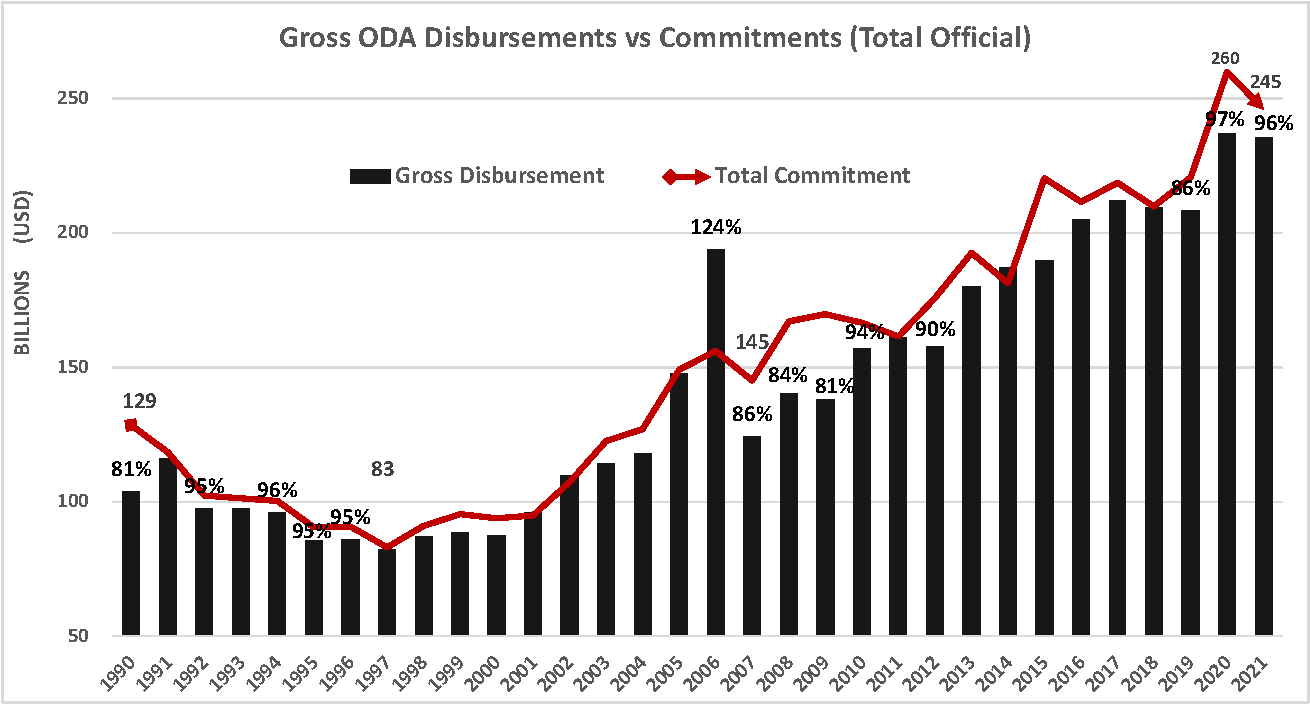
\includegraphics[width = 0.7\textwidth]{Figures/ODA_Graphs/Dibs_VS_Commit.pdf}
    \label{Disbursement Vs Commitment}
\caption*{\footnotesize{Note: Both ODA commitment and disbursement are in 2021 constant price, in USD billion. Author's computation with data from \textcite{oecd_Data_2023}.}}
\end{figure}

%%%%%%%%%%%%%%%%%%%%%%%%%%%%%%%%%%%%%%%%%%%%%%%%%%%%%%%%%%%%%%%%%%%%
% ODA commitment by sectors  						yes
 Figure \ref{fig:ODA sectors commitment} further illustrates the distribution of ODA commitments across sectors.Notably, the social infrastructure and humanitarian sectors emerge as primary recipients of ODA commitments. The Humanitarian sector witnessed substantial growth in committed ODA, escalating from 1\% (1.7 billion USD) of total ODA in 1990 to 16\% in 2021, signifying a remarkable 1,600\% increase over the data period. Simultaneously, the social infrastructure sector rose from 30 billion USD (24\%) in 1990 to a peak of 103 billion USD (43\%) in 2007, subsequently experiencing a gradual reduction to 42\% in 2019. It's crucial to note that while the percentage decreased, the absolute value continued to show an upward trend. This reduction in percentage is attributed to the overall increase in total ODA commitments over the years. The surge in commitments to the humanitarian and social infrastructure sectors since the 2000s can be linked to the MDGs and the subsequent SDGs, reflecting global commitments to addressing poverty and social challenges. Similarly, commitment to economic infrastructures also increased in absolute value starting from 22.5 billion USD or 18\% of the total ODA commitment in 1990 to 35.2 billion or 14\% in 2021. Therefore, considering the pattern of commitments, particularly to the humanitarian and social infrastructure sector, it is logical to consider the total ODA for measuring the effectiveness of ODA.

\begin{figure}[ht]
\captionsetup{justification=justified,singlelinecheck=false}
\caption{\textit{Sectoral ODA Commitments}}
    \centering 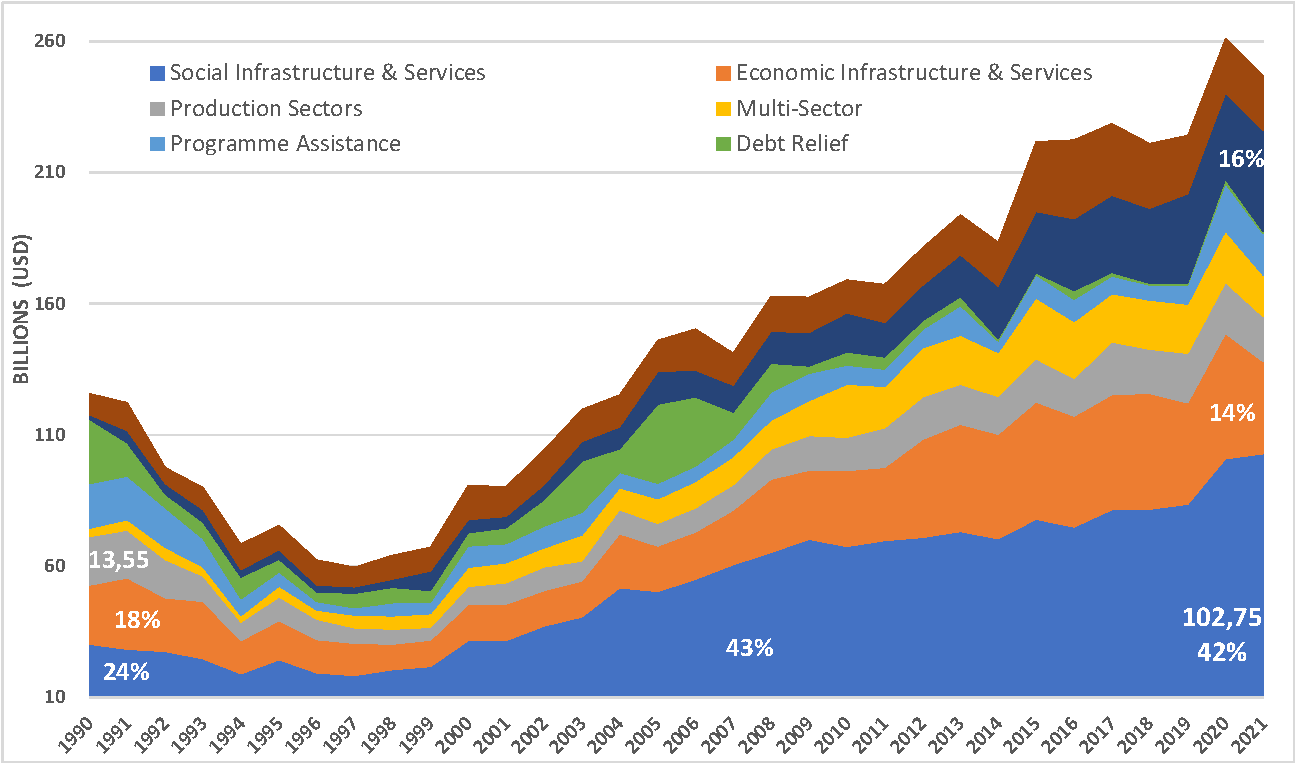
\includegraphics[width = 0.7\textwidth]{Figures/ODA_Graphs/Sector_class.pdf}
    \label{fig:ODA sectors commitment}
    \caption*{\footnotesize{Note. Data for sectoral allocation of ODA is only available for commitment, and not disbursement. However, given the closeness of the two, commitment is a valid proxy for disbursement. Data is in USD billion 2021 constant price, Author's computation with data from \textcite{oecd_Data_2023}}}
\end{figure}

%%%%%%%%%%%%%%%%%%%%%%%%%%%%%%%%%%%%%%%%%%%%%%%%%%%%%%%%%%%%%%%
% Social Infrastructure subsector of ODA 					yes
Particularly crucial to this thesis is the allocation to social infrastructure, which include the health subsector. Figure \ref{fig:Subsector of Social Infrastructure} illustrates the evolving interest and commitment of donors over time in the six subsectors of the social infrastructure sector. Notably, ODA to the health sector grew consistently both in relative and absolute terms, from 13\% in 1990 to 31\% of the total social infrastructure sector by 2021. This growth is most visible in Covid-19 pandemic, with health commitments increasing by over 10\% between 2019 and 2021. The emphasis on health extends to the reproductive health and population subsector, which also experienced substantial growth, rising from 4\% of the total commitment to 12\% in 2021. However, ODA's commitment to water sanitation and education has declined, indicating a shifting pattern in donors' interests over time. Support for government budgets reached its zenith in 2004, constituting 35\% of the total commitment, but has gradually decreased to 22\% by 2021.

\begin{figure}[ht]
\captionsetup{justification=justified,singlelinecheck=false}
\caption{\textit{Evolution of ODA in Social Infrastructure Sector(ODA Commitments)}}
    \centering 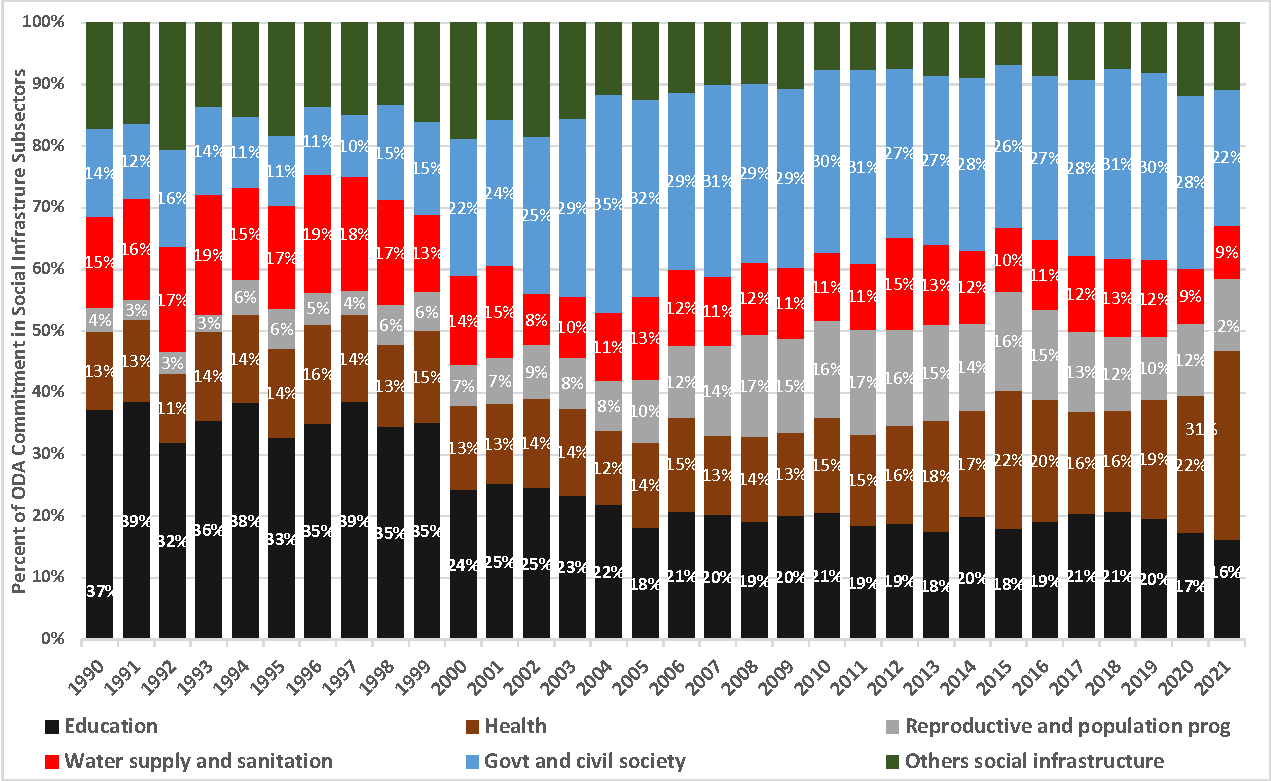
\includegraphics[width = 0.7\textwidth]{Figures/ODA_Graphs/Subsectors_soc_inf.pdf}
    \label{fig:Subsector of Social Infrastructure}
    \caption*{\footnotesize{Despite growth in health ODA, unspecified social infrastructure ODA is high, as shown in Fig \ref{fig:Subsector of Social Infrastructure}. Therefore, the thesis combines the social infrastructure ODA with the total Net ODA for the main analysis. Author's computation with Data from \textcite{oecd_Data_2023}}}
\end{figure}

%%%%%%%%%%%%%%%%%%%%%%%%%%%%%%%%%%%%%%%%%%%%%%%%%%%%%%%%%%%%%%%%%%%%%%%%%%
\paragraph{\quad \quad \textit{2.1.2.2  ODA Characterization by Donors}}
% DAC donors and non-dac donors   Evolution of Net ODA disbursement yes 
\paragraph{}Figure \ref{fig:ODA by donors} illustrates the distribution of ODA donors, categorizing them into DAC (Development Assistance Committee) donors, which are OECD member countries providing bilateral ODA to developing nations, and non-DAC bilateral and multilateral net ODA donors. DAC countries consistently play a significant role as ODA donors, contributing around 67\% of the total ODA. This percentage was equivalent to 61.4 billion in 1990 and increased to 63\% or 129.3 billion in 2021. While the DAC bilateral ODA declined in 2014, it still constituted a substantial portion, accounting for 67\% or 92 billion of the total. Multilateral donors constituted 20\% of ODA in 1990, growing to 28\% or 57.4 billion in 2021. In contrast, non-DAC ODA had a relatively negligible share, ranging from 10\% in 1990 to fluctuating between 2\% and 5\% during the 2000s. Notably, there has been significant growth in non-DAC countries' ODA since 2010, reaching 9\% or 19.36 billion.

\begin{figure}[ht]
\captionsetup{justification=justified,singlelinecheck=false}
\caption{\textit{Evolution of Net ODA Disbursement by Donors}}
    \centering 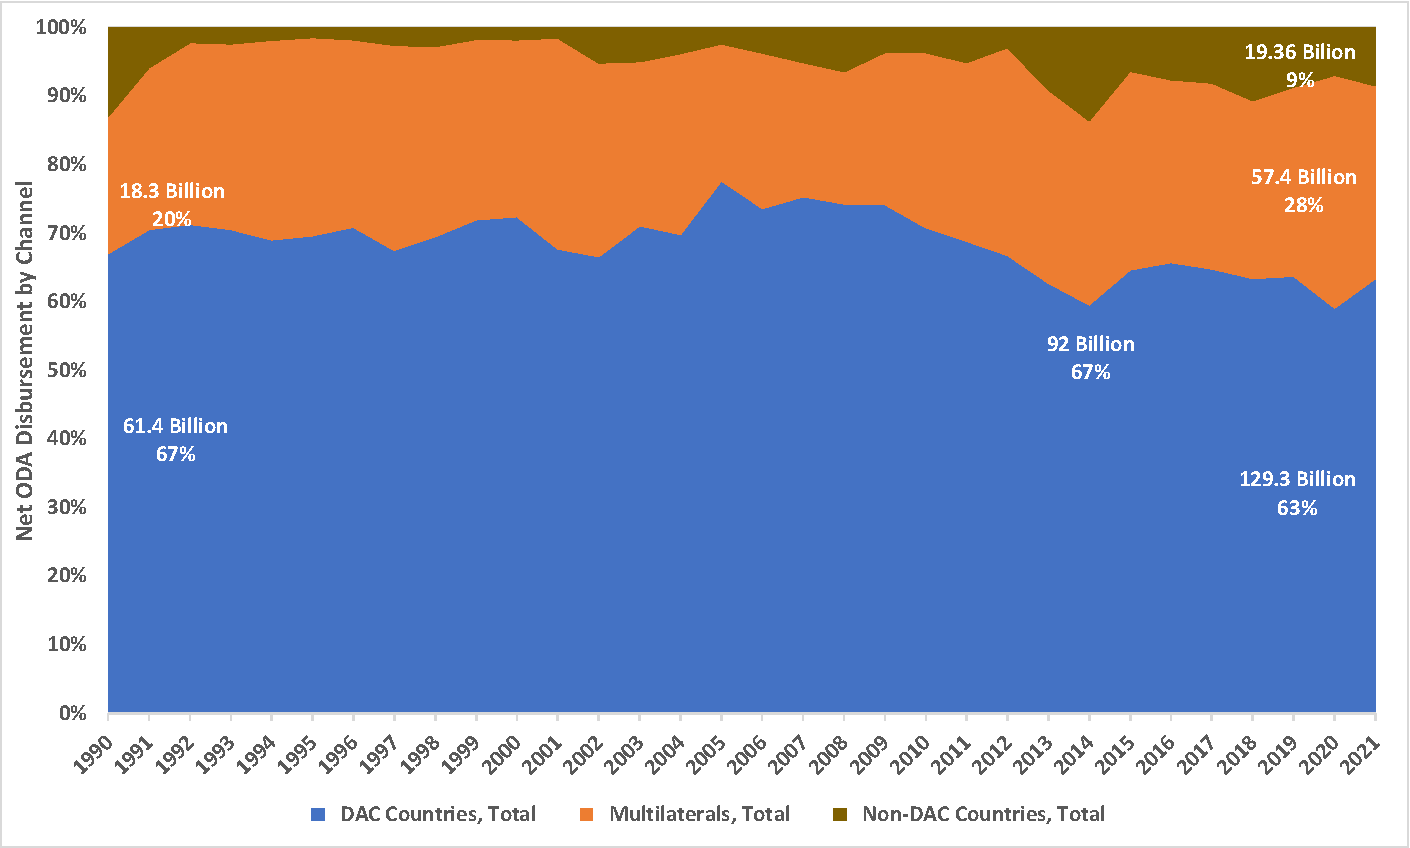
\includegraphics[width = 0.7\textwidth]{Figures/ODA_Graphs/Evolution_Net_ODA.pdf}
    \caption*{\footnotesize{Note. Percentage is the author's computation using Net ODA in 2021 constant price, data from \textcite{oecd_Data_2023}}}
    \label{fig:ODA by donors}
\end{figure}

%%%%%%%%%%%%%%%%%%%%%%%%%%%%%%%%%%%%%%%%%%%%%%%%%%%%%%%%%%%%%%%%%%%%%%%%%%%%%%H%ighest Net ODA Donors among DAC 			yes

In Figure \ref{fig:Highest ODA donors}, among the DAC donors, the United States (US) has consistently been the highest donor since 1990, allocating 25\% or 15 billion USD of the total DAC ODA. The US experienced a significant decline in ODA in 1996, impacting the global ODA allocation. Despite being a major donor, the US reached a record low of 7.9 billion or 17\% during the early 1990s recession. Subsequently, US ODA steadily increased, reaching 34 billion or 34\% of DAC's total ODA before declining again due to the 2008 recession. Germany, on the other hand, initially the fourth-highest DAC donor with 7 billion or 12\% of the total DAC in 1990, ascended to the second-highest donor in 2006, surpassing France and Japan. By 2016, Germany disbursed approximately 20\% or 23 billion of the total DAC. France and Japan's ODA remained relatively stable, fluctuating between 13\% and 14\% of the total DAC in 1990 to 8\% and 9\% in 2021. Notably, Germany's ODA exhibited relative stability and predictability over the years, with fewer cyclical changes compared to the USA.

\begin{figure}[ht]
\captionsetup{justification=justified,singlelinecheck=false}
\caption{\textit{Highest Donors of Net ODA Disbursement in DAC Countries}}
\vspace{4pt}
    \centering 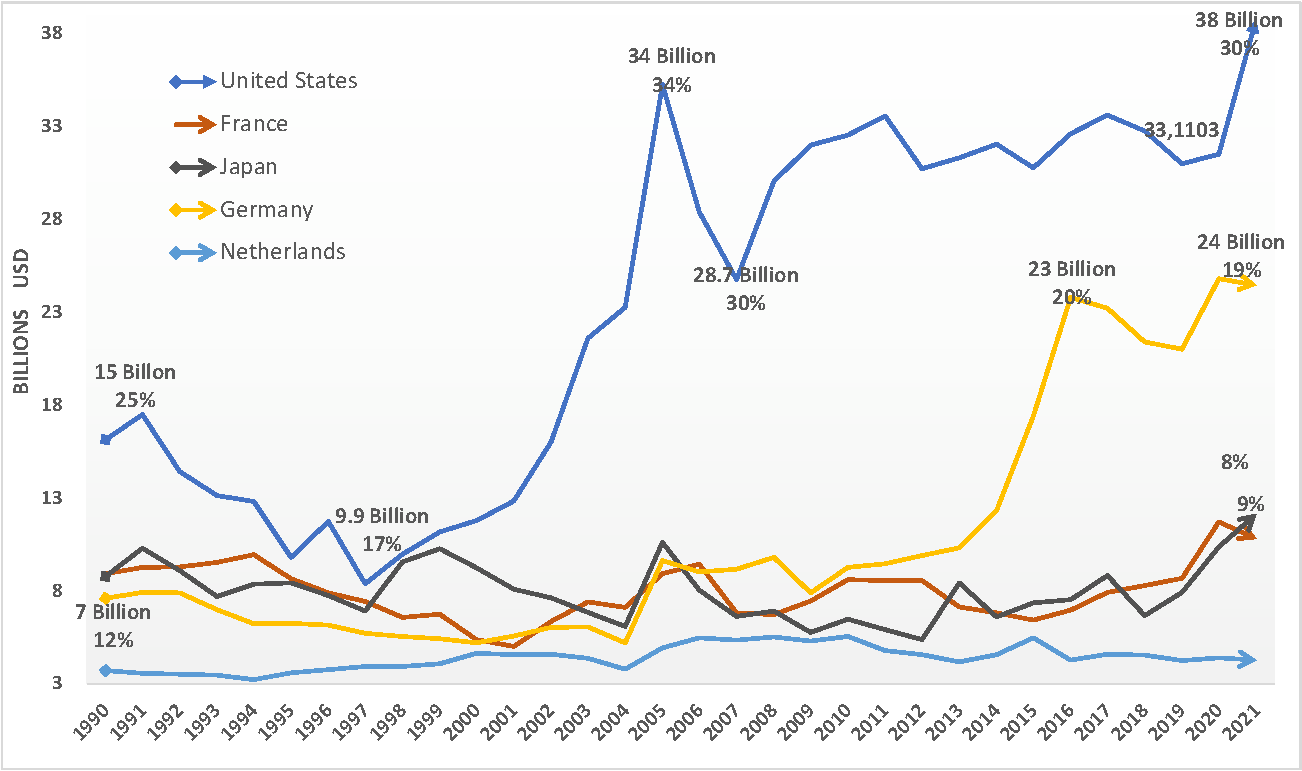
\includegraphics[width = 0.7\textwidth]{Figures/ODA_Graphs/Top_DAC_Donors.pdf}
    \caption*{\footnotesize{Net ODA in 2021 constant price billion USD. Author's computation with sata from \textcite{oecd_Data_2023}}}
    \label{fig:Highest ODA donors}
\end{figure}

%%%%%%%%%%%%%%%%%%%%%%%%%%%%%%%%%%%%%%%%%%%%%%%%%%%%%%%%%%%%%%%%%%
\paragraph{\quad \quad \textit{2.1.2.3 ODA Characterization by Recipients}}
% Time and regional distribution of Net ODA by continents    yes
\paragraph{} Figure \ref{fig:ODA by continent} presents the distribution of ODA recipients by continents. Accordingly, the African continent has consistently been the highest recipient of Net ODA, with the estimated amount increasing from 42 billion USD or 46\% of the total ODA in 1990 to 75 billion or 37\% in 2021. Asia follows, with the amount growing from 26 billion or 29\% in 1990 to 54 billion or 26\% in 2021. Although both Africa and Asia's ODA grew relatively close, with an increase of 28 billion over 30 years, Africa's ODA reduced in relative terms compared to Asia.

\begin{figure}[ht]
\captionsetup{justification=justified,singlelinecheck=false}
\caption{\textit{Recipients of ODA by Continents}}
\vspace{4pt}
    \centering 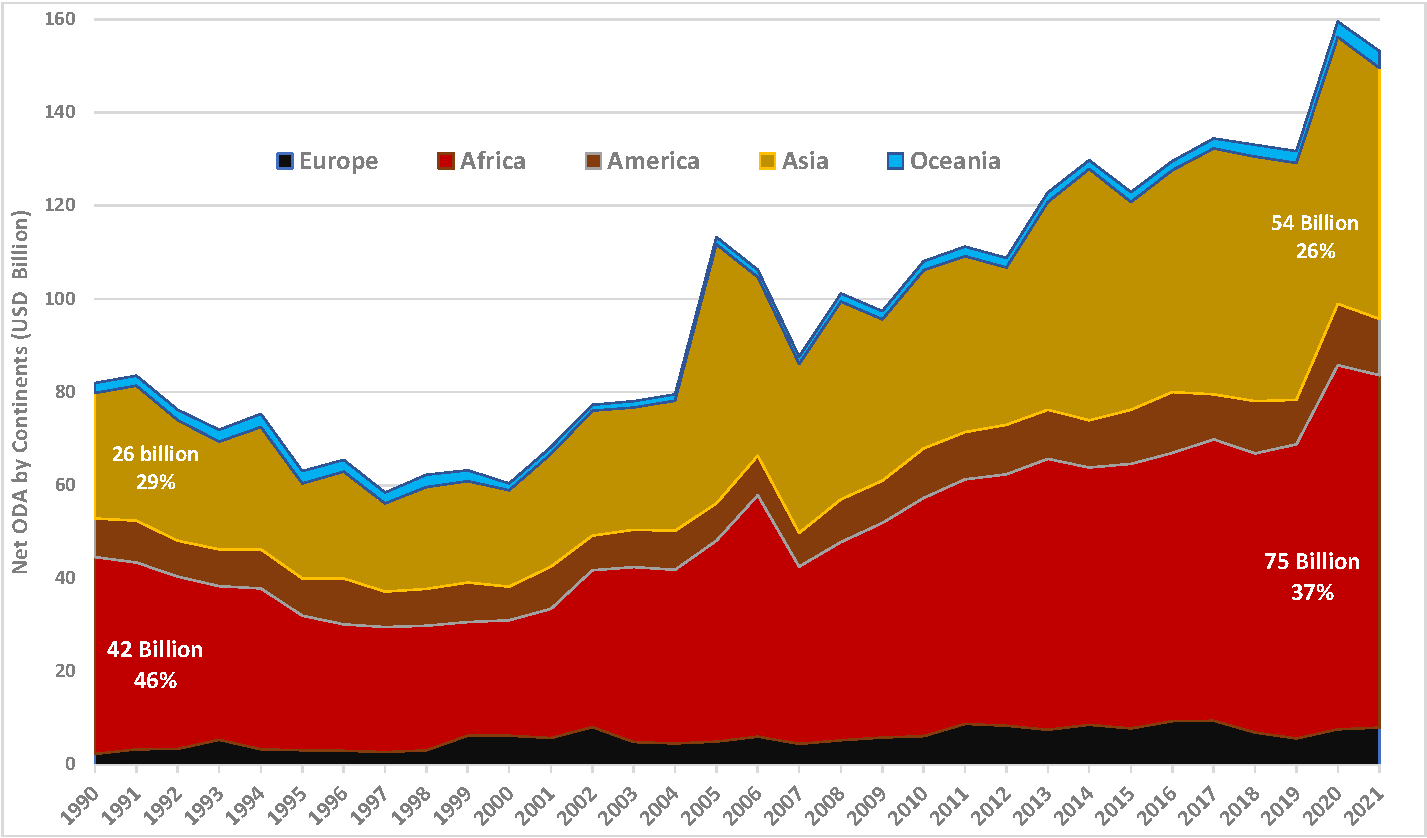
\includegraphics[width = 0.7\textwidth]{Figures/ODA_Graphs/Dist_ODA_by_continents.pdf}
    \caption*{\footnotesize{Note: Net ODA in 2021 constant price billion USD. Author's computation, with data from \textcite{oecd_Data_2023}}}
    \label{fig:ODA by continent}
\end{figure}


However, a more detailed examination at the country level, as depicted in Appendix Figure \ref{fig:ODA highest recipient}, reveals a nuanced scenario. Only three African and seven Asian countries are among the top ten recipients of Net ODA. Iraq leads as the highest net ODA recipient, averaging 3.2 billion USD, closely followed by Afghanistan with 3.1 billion. Notably, conflict-affected countries such as Iraq, Afghanistan, Congo DRC, and Ethiopia account for a significant volume of ODA. Additionally, India ranks as the seventh-highest net ODA recipient, followed by Bangladesh and Tanzania.





%ODA dependency \footnote{ODA dependency defined as the percentage of Net ODA received per recipient GNI.}, as used in other studies \textcite{temple_aid_2010}, provides a magnified view of the aid landscape across countries and regions. This is illustrated in Figure \ref{fig:ODA Dependency by region} and Appendix Figure \ref{fig:aid dependency}. Accordingly, all the regions are statistically different in their level of aid dependency. These figures reveal that Sub-Saharan Africa (SSA) is the highest aid-dependent region, notable highly aid-dependent countries in SSA include Ethiopia, Mozambique, Rwanda, Liberia, and the Central African Republic, as shown in Appendix Figure \ref{fig:aid dependency}.



\begin{figure}[ht]
\captionsetup{justification=justified,singlelinecheck=false}
\caption{\textit{Regional Comparison of Aid Dependency: ODA per Countries' GNI}}
    \centering 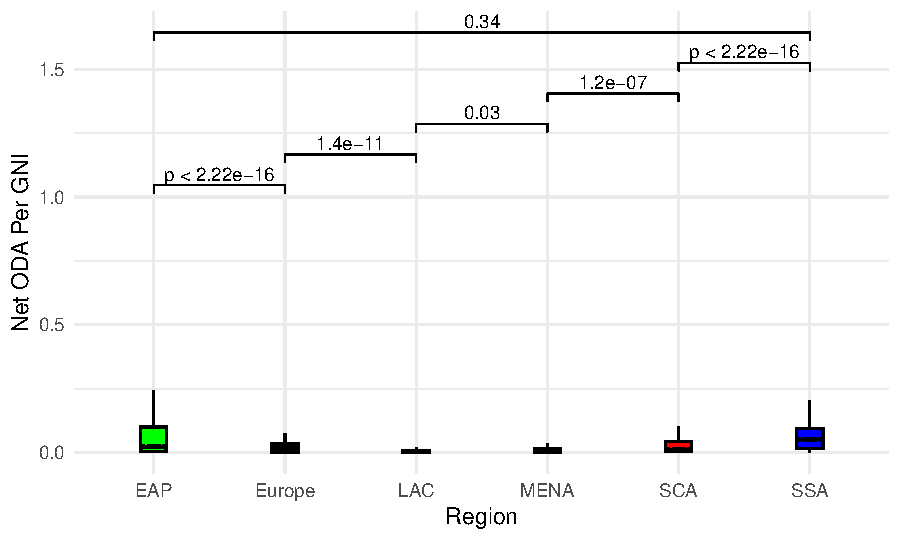
\includegraphics[width = 0.7\textwidth]{Figures/ODA_Graphs/ODA_GNI_boxplt.pdf}
    \caption*{\footnotesize{Note: ODA is logged to reduce outliers. The P-values are derived from the t-test, for statistical differences among the regions. Author's compuataion with data from \textcite{oecd_Data_2023}}}
    \label{fig:ODA Dependency by region}
\end{figure}

ODA dependency, defined as the percentage of Net ODA received per recipient GNI, provides a nuanced view of the aid landscape across countries and regions, as used in other studies \textcite{temple_aid_2010}. This is highlighted in Figure \ref{fig:ODA Dependency by region} and Appendix Figure \ref{fig:aid dependency}. All regions show statistically significant differences in their levels of aid dependency. Sub-Saharan Africa (SSA) emerges as the highest aid-dependent region, particularly in countries such as Ethiopia, Mozambique, Rwanda, Liberia, and the Central African Republic, as depicted in Appendix Figure \ref{fig:aid dependency}. Similarly, the South and Central Asia (SCA) and East Asia and Pacific (EAP) regions exhibit high and comparable levels of aid dependency, influenced particularly by small countries such as Marshall Islands and Tuvalu. Despite the relatively low incidence of ODA dependency in the Middle East and North Africa (MENA) region, war-torn countries like Iraq and Syria demonstrate extreme values of dependency on a global scale.



%%%%%%%%%%%%%%%%%%%%%%%%%%%%%%%%%%%%%%%%%%%%%%%%%%%%%%%%%%%%%%%%%%%%%%%%%%%%%%%%%%%%%%%%%%%%%%%%%%%%%%%%%%%%%
\subsection*{2.2 Health Outcome}
\addcontentsline{toc}{subsection}{2.2 Health Outcomes}
\subsubsection*{\quad 2.2.1 Conceptualizing Health Outcomes}
\addcontentsline{toc}{subsubsection}{2.2.1 Conceptualizing Health Outcomes}

\paragraph{}The term "health outcome" encapsulates two constructs: "outcome" and "health." Both Oxford and Cambridge dictionaries define an outcome as a consequence, a result or effect of an action or event \parencite{cambridge_dictionary_outcome_2023, oxford_dictionary_outcome_nodate}. Thus, an outcome could be semantically attributed to the consequence of an action(s) in any context by any capable being. The concept of “health”, on the other hand, is pluralistic and has evolved. Historically, health was perceived in terms of physiological functioning: a harmony between the human mind and social environment \parencite{svalastog_concepts_2017}. 

A more holistic view, conceptualized within the bio-psychosocial framework, is reflected in the WHO 1948 constitution. According to it, health is defined as "the state of complete physical, mental, and social well-being and not merely the absence of disease or infirmity" \parencite{who_constitution_1946}. This definition underscores social welfare as a crucial component of human health, acknowledging the impact of living and working conditions on health \parencite{svalastog_concepts_2017}. A notable linkage between health and economic conditions is traceable to the health production theory, which emphasizes the relevance of health capital to economic capacity \parencite{grossman_concept_1972}. Reflecting on the capability perspective with the temporal dynamics of health, \textcite{huber_how_2011} define health as the ability to adapt and self-management, particularly to handle social, physical and emotional problems. Also, nutrition has become an essential aspect of health over time \parencite{gamble_why_2008} \footnote{According to the Food and Agriculture Organization (FAO), nutrition interacts with health in three important ways: increased body demand for nutrition to maintain homeostasis; reduction of food intake; and waste from vomiting \parencite{fao_study_1996}}. 

Therefore, the thesis draws insight from Shafa and colleagues' \parencite{shafa_assessment_2023} definition of health outcomes. Accordingly, health outcome is defined as tool(s) for assessing the impact of care or intervention on people's health situation. Since health is multidimensional, health metrics are equally complex. Health outcome metrics may be include indicators such as life expectancy, child mortality, and morbidity \parencite{shafa_assessment_2023} as well as composite indices i.e. Universal Health Coverage (UHC) index. SDG 3, focusing on health and well-being provides international indicators critical for assessing health outcomes and crucial for this study. The six composite health dimensions are discussed below. 
% Another uniqueness of this thesis is the incorporation of nutrition to measure health outcomes, accommodating regional differentials in the burden of health. This section further explores the distribution of crucial health outcome indicators across countries and regions.

%%%%%%%%%%%%%%%%%%%%%%%%%%%%%%%%%%%%%%%%%%%%%%%%%%%%%%%%%%%%%%%%%%%%%%%%
\subsubsection*{\quad 2.2.2 Characterizing Health Outcomes in Developing Countries}
\addcontentsline{toc}{subsubsection}{2.2.2 Statistical Characterization of Health Dimensions}
This thesis employs a comprehensive approach to measure health outcomes by considering the multidimensionality of health. It incorporates 25 unique indicators from SDG 2 and 3 for health and malnutrition, respectively. These indicators are employed to create six composite health dimensions: Reproductive Fatality and Teen Pregnancy (RFTP), Burden of Infection and Diseases (BID), Burden of Mental Problems (BMP), Malnutrition, Environmental Death, and Health System Capacity and Responsiveness (HSCR). All unique indicators are standardized to ensure comparability (see the procedure in Appendix B.1). Figure \ref{fig:combined_Box_plot} displays the six health dimensions, with each panel representing one dimension. The associated p-values, derived from t-tests, determine the significant differences in health dimensions among regions, to justify inaccuracy of using narrow health indicators to assess ODA effectiveness.


%\caption*{\footnotesize{Note: Each panel of the graph represents each of the six composite health dimensions, created using equal weightings. Plot A contains Reproductive fatality and Teen Pregnancy (RFTP), Plot B shows Burden of Infection and diseases (BID). Plot C illustrates the Burden of Mental Problems (BMP). Plot D represents Malnutrition, Plot E on Environmental Death and Plot F for Health System Capacity and Responsiveness (HSCR). See respective indicators for various health dimensions in Appendix Table \ref{Tab::health indicators}. Lines in the middle of boxes indicate the median, the bottom and top of each box are the 25th and 75th quartile respectively, while whiskers represent the 95\% Confidence Interval (CI). The kernel density curve indicates the distribution of specific health dimensions within respective regions. Author's computation, data from \textcite{unsdg_sustainable_2023, wdi_world_2023}}}
 
Starting from RFTP, in Figure \ref{fig:combined_Box_plot} Plot A, all regions are significantly different. SSA region has the highest RFTP, densely distributed among its countries, with specific countries such as Guinea-Bissau, Sierra Leone, Chad, Liberia, Rwanda, and Nigeria ranking among the worst (see Appendix B.2 Figure \ref{fig:combined_scat_plot} for country-level details). SCA also shows moderately high RFTP, but many countries within the region are below its median. Europe, on the other hand, has the lowest reproductive fatalities (RFTP), with most countries clustered around its median. In Plot B of Figure \ref{fig:combined_Box_plot}, infection and disease (BID) also significantly vary across the regions. Notably, both SSA and SCA have the worst BID cases, densely distributed among their countries. India, Kiribati, Lesotho, Swaziland, Zimbabwe, Ethiopia, and the Central African Republic (CAF) have the highest BID, as shown in Appendix B.2 Figure \ref{fig:combined_scat_plot}.


\begin{landscape}
    \begin{figure}[ht]
\captionsetup{justification=justified,singlelinecheck=false}
\caption{\textit{Composite Health Dimensions Across Regions of Developing Countries}}
    \centering 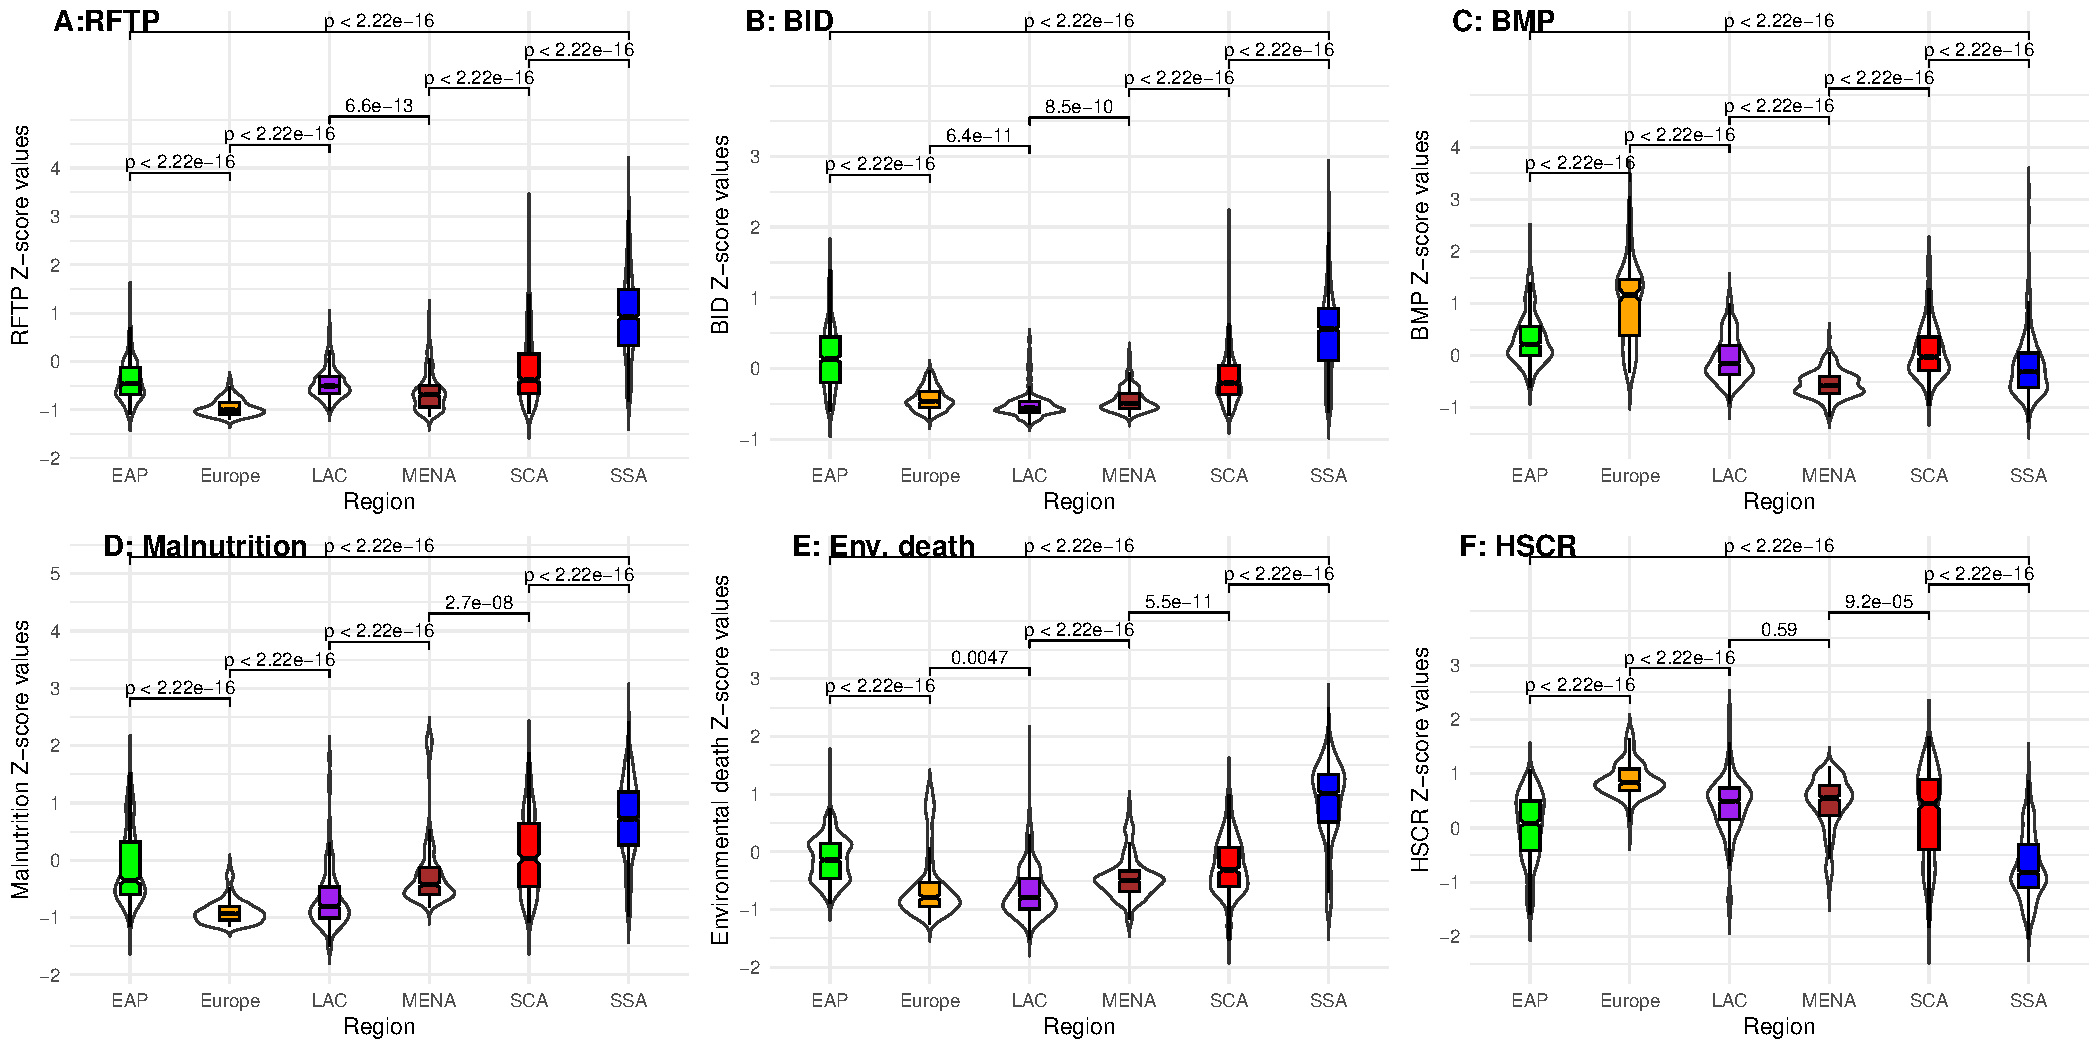
\includegraphics[width = 1.65\textwidth]{Figures/Health_Outcome_Graph/Combined_Boxplt_2.pdf}
    \caption*{\footnotesize{Note: Each panel in the graph corresponds to one of the six composite health dimensions, created with equal weightings. Plot A features Reproductive Fatality and Teen Pregnancy (RFTP), Plot B depicts the Burden of Infection and Diseases (BID), Plot C illustrates the Burden of Mental Problems (BMP), Plot D represents Malnutrition, Plot E focuses on Environmental Death, and Plot F addresses Health System Capacity and Responsiveness (HSCR). See specific health indicators for each health dimension in Appendix Table \ref{Tab::health indicators}) and procedure in Appendix B.1. Author's computation, data sourced from \textcite{unsdg_sustainable_2023, wdi_world_2023}.}}
    \label{fig:combined_Box_plot}
\end{figure}
\end{landscape}


Mental problem, depicted in Figure \ref{fig:combined_Box_plot} Plot C as Burden of Mental Health (BMP), is highest in Europe and widely dense among its countries. Specific European countries with the highest incidence include Ukraine, Belarus, Serbia, and Croatia. BMP shows significant differences across all regions, with MENA and SSA having the lowest cases, and most countries in these regions falling below their respective regional median value. For the malnutrition health dimension (Plot D in Figure \ref{fig:combined_Box_plot}), all regions exhibit statistically significant differences, with the highest cases in SSA, SCA, and EAP. SSA has the highest malnutrition, densely distributed among its countries. While SCA and EAP also show high malnutrition, the situation tends to be more spread in SCA countries than in EAP.

Environmental death, presented in Figure \ref{fig:combined_Box_plot} Plot E, significantly varies across regions, with the highest in SSA. SCA and EAP also exhibit very high environmental death, but with different distribution patterns. SCA countries have a high density below the region's median, while most EAP countries are above their region's median value. Finally, Health System Capacity and Responsiveness (HSCR) in Figure \ref{fig:combined_Box_plot} Plot F show significant differences across regions, except between LAC and MENA regions. Europe has the highest HSCR, with most countries clustering in the 75th quartile of its region. While both LAC and MENA regions also have high health capacity, SSA stands out with the poorest health system among the regions compared.




%Considering the multidimensionality of health, this thesis adopts a comprehensive approach to measuring health outcomes, incorporating 25 unique indicators from SDG 2 and 3 for health and malnutition, respectively. All indicators are used to create six composite health dimensions: Reproductive Fatality and Teen Pregnancy (RFTP), Burden of Infection and Diseases (BID), Burden of Mental Problem (BMP), Malnutrition, environmental death, and Health System Capacity and Responsiveness (HSCR). Specific indicators within each dimension are standardized before creating dimension indices to ensure comparability (see procedure in Appendix B.1). The six health dimensions are presented in Figure \ref{fig:combined_Box_plot}, with each panel representing each health dimension. The p-values are derived from t-test showing whether specific health dimensions is significantly different among regions. This is essential to invalidate the use of narrow health indicators in assessing ODA effectiveness. 


%As shown in Figure \ref{fig:combined_Box_plot} Plot A, RFTP p-value is statistically different across the regions. Specifically, Sub-Saharan Africa (SSA) has the highest RFTP and densely distributed among its countries, with specific countries like Guinea-Bissau, Sierra Leone, Chad, Liberia, Rwanda, and Nigeria ranking among the worst (see Appendix B.2 Figure \ref{fig:combined_scat_plot} for country level). While RFTP is also moderately high in South and Central Asian (SCA) region, many countries are below the region median value. Europe has the lowest reproductive fatalities, with most countries clustered around the median index value, as indicated by the bulge density. In the same Figure \ref{fig:combined_Box_plot} plot B illustrate between region comparison of BID. Accordingly, all regions are statically different in their burden of infections and diseases, value of all sample comparison \textless 1\%. Furthermore, despite regions being closely related on this dimension, both SSA and SCA have the worst BID cases, and densely among their countries, with India, Kiribati, Lesotho, Swaziland, Zimbabwe, Ethiopia, and the Central African Republic (CAF) having the highest, as shown in Appendix B.2 Figure \ref{fig:combined_scat_plot}. 


 %Mental health is equally an essential aspect of human health. Unlike reproductive fatality (RFTP) and infection and diseases (BID) health dimensions, Figure \ref{fig:combined_Box_plot} plot C shows Burden of Mental Health (BMP) is the highest in Europe and, widely dense among its countries. In Appendix Appendix Figure B.2 Figure \ref{fig:combined_scat_plot}, Specific European countries with the highest incidence include Ukraine, Belarus, Serbia, and Croatia. Furthermore, BMP is significantly different across all regions, with Middle East and North Africa (MENA) and SSA having lowest cases, with most countries in the regions below the median value of their respective regional median values. In the malnutrition health dimension, Figure \ref{fig:combined_Box_plot} plot D, all the regions are statistically different, with the highest cases in SSA, SCA and EAP. Specifically, malnutrition is the highest in SSA, and densely distributed among its countries. Malnutrition is also high for SCA and EAP regions, however,  the situation tend to more spread in SCA countries than EAP.


%Environmental death, in Figure \ref{fig:combined_Box_plot} plot E, also significantly vary across, albeit, the level of significance vary. As illustrated in plot E, environmental death is the highest in SSA and the distribution reflects other health dimensions. Both SCA and EAP equally exhibit very high environmental death, but SCA countries have a high density below the region's median, while most EAP countries are above their region's median value. Regardless of the intensity of health problems, health system capacity and responsiveness (HSCR) is essential to handle health problems when arise. As shown in Figure \ref{fig:combined_Box_plot} plot F, HSCR is significantly different across regions with p-value \textless{} 1\% except between LAC and MENA regions. Europe has the highest HSCR, with most of its countries clustering in the 75th quartile of its region. While both LAC and the MENA regions are also high in health capacity, with similar similar distribution shapes among their respective countries, SSA has the poorest health system among the regions compared. 




%\begin{figure}[ht]
%\captionsetup{justification=justified,singlelinecheck=false}
%\caption{\textit{Reproductive Health Risk and Mortality Dimension}}
%    \centering 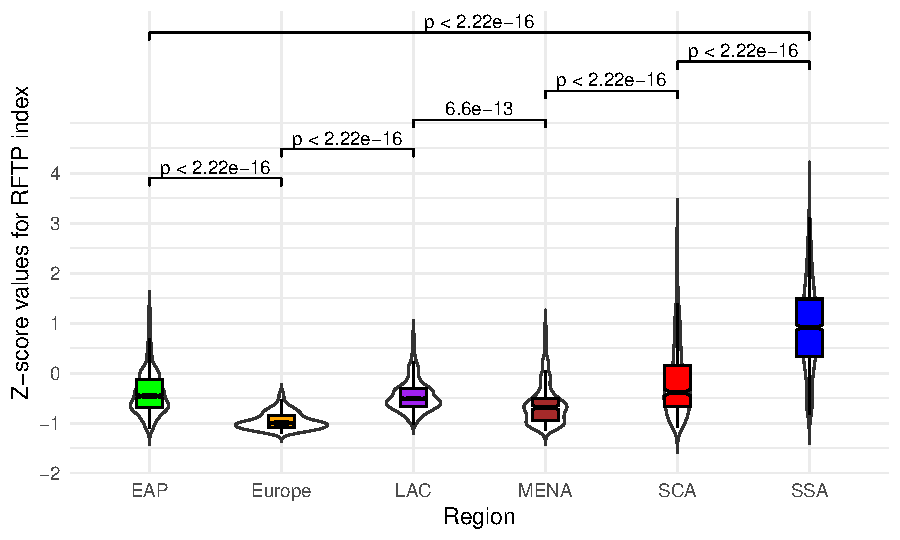
\includegraphics[width = 0.8\textwidth, height = 7cm]{Figures/Health_Outcome_Graph/Reprod_Risks_boxplt.pdf}
 %   \caption*{\footnotesize{Note. Reproductive health risk and mortality index comprises four indicators: maternal, under-5 child and neonatal mortality, and adolescent pregnancy incidence (10 to 19 years) access across the regions of interest. Author's computation, data from \textcite{unsdg_sustainable_2023, wdi_world_2023}}}
  %  \label{fig:reproduction boxplot}
%\end{figure}


%1.65


%

% Figure: Burden of Infection and diseases 


% Figure: Mental Health Problem

%\begin{figure}[ht]
%\captionsetup{justification=justified,singlelinecheck=false}
%\caption{\textit{Mental Health Dimension}}
 %   \centering 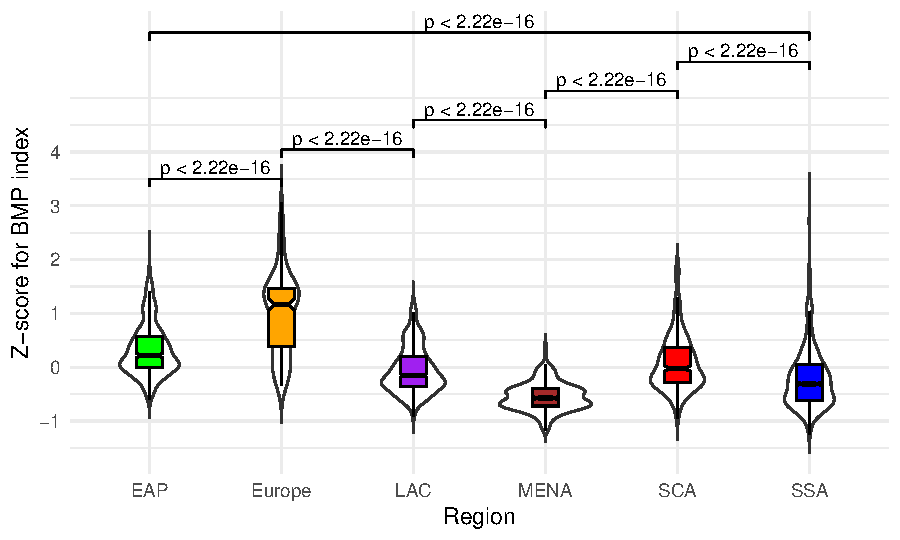
\includegraphics[width = 0.8\textwidth, height = 7cm]{Figures/Health_Outcome_Graph/Mental_Hth_boxplt.pdf}
  %  \label{fig:Mental health}
   % \caption*{\footnotesize{Note. Mental health dimension is derived from three indicators: mortality by suicide, alcohol per capita consumption, and population incidence of tobacco. P-value derived from two-way paired t-test. All regions are significantly different at p-value \textless{} 1\%. Author's computation, data from \textcite{unsdg_sustainable_2023, wdi_world_2023}}}
%\end{figure}


%\begin{figure}[ht]
%\captionsetup{justification=justified,singlelinecheck=false}
%\caption{\textit{Burden of Infection and Diseases Dimension}}
 %   \centering 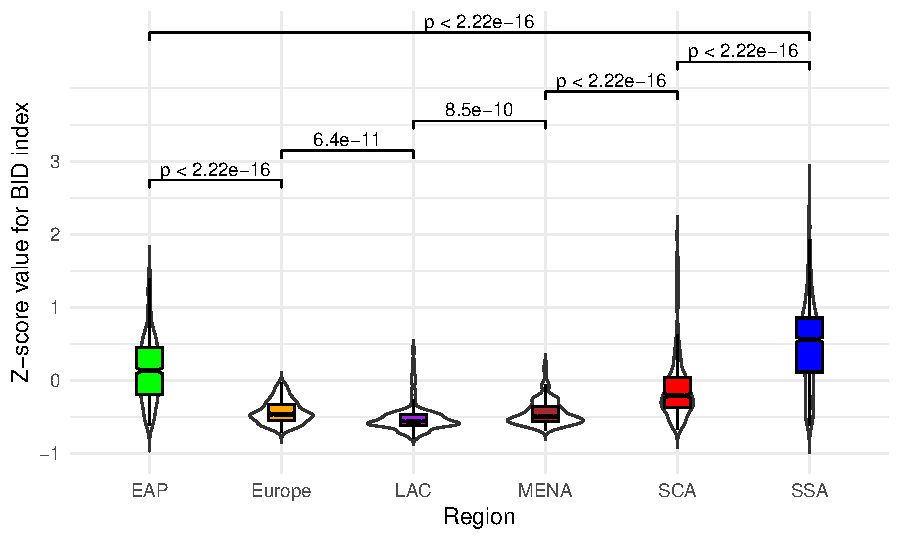
\includegraphics[width = 0.8\textwidth, height = 6cm]{Figures/Health_Outcome_Graph/Burd_Infs_boxplt.pdf}
  %  \label{fig:Infection burden}
   % \caption*{\footnotesize{Note. The burden of infection and diseases (BID) five indicators: new HIV cases, population tuberculosis incidence, malaria incidence, hepatitis-B among under-5, tropical diseases and mortality rate from non-communicable diseases \footnote{Example of Non-communicable disease (NDC) are cardiovascular disease, cancer, diabetes or chronic respiratory disease}.  P-value derived from two-way paired t-test. All regions are significantly different at p-value \textless{} 1\%. Author's computation, data from \textcite{unsdg_sustainable_2023, wdi_world_2023}}}
%\end{figure}



% Figure: Incidence of Malnutrition
%In malnutrition dimension, Figure \ref{fig:malnutrition index}, all the regions have statistically different levels of malnutrition. Specifically, SSA has the highest malnutrition intensity among all the regions, with most countries in the region below its regional 75th quartile. Malnutrition intensity is also high for SCA and EAP regions, however, the density distribution varies across the two. While malnutrition intensity is widely spread in SCA countries, most EAP countries are below its regional median value. Both the LAC and the MENA regions exhibit moderate malnutrition, while Europe has the lowest intensity (see Appendix 6 for country comparison).
%\begin{figure}[ht]
%\captionsetup{justification=justified,singlelinecheck=false}
%\caption{\textit{Dimension Index for Malnutrition}}
 %   \centering 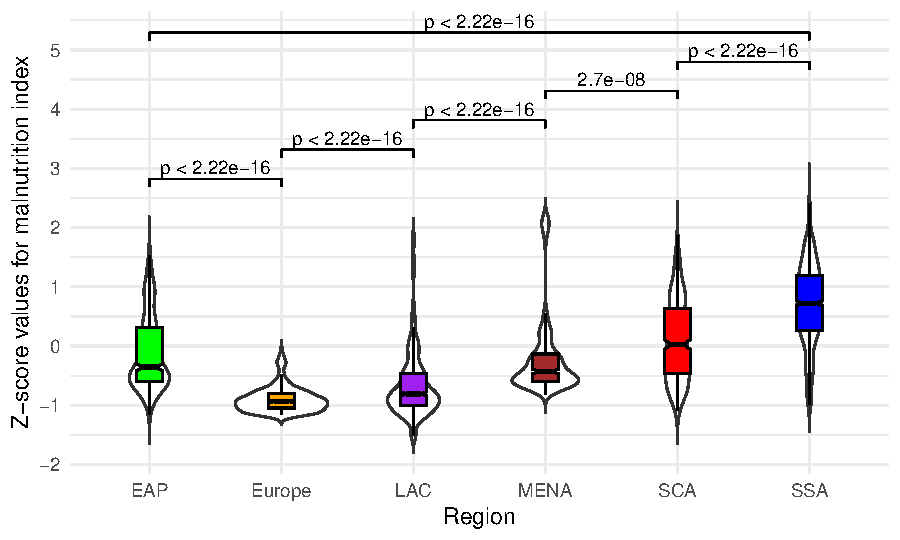
\includegraphics[width = 0.8\textwidth, height = 7cm]{Figures/Health_Outcome_Graph/Malnutrition_boxplt.pdf}
  %  \label{fig:malnutrition index}
   % \caption*{\footnotesize{Note. Malnutrition dimension comprises three indicators specifically from SDG 2: Percentage of 15 - 49 years women with anemia, population undernutrition, and under-5 children moderately or severely stunted. Author's computation, data from \textcite{unsdg_sustainable_2023, wdi_world_2023}.}}
%\end{figure}
% Figure: Environmental Induce Death
%Unlike previous health dimensions, not all regions are statistically different in environmental death. As illustrated in Figure \ref{fig:Env mortality}, while other regions are statistically different (p-value \textless{} 5\%), Europe and Latin America (LAC) are similar in environmental death (p-value \textgreater{} 5\%). Specifically,  SSA has the highest environmental death and is statistically different from all other regions. However, most of its countries experience environmental mortality above the region's median value. Both SCA and EAP equally exhibit very high environmental mortality, but the distribution among countries differs between the two regions. SCA countries have a high density below the region's median, while most EAP countries are above their region's median value. Environmental mortality density is similar across Europe, LAC, and MENA regions.

%\begin{figure}[ht]
%\captionsetup{justification=justified,singlelinecheck=false}
%\caption{\textit{Dimension Index for Environmental Related Mortality}}
 %   \centering 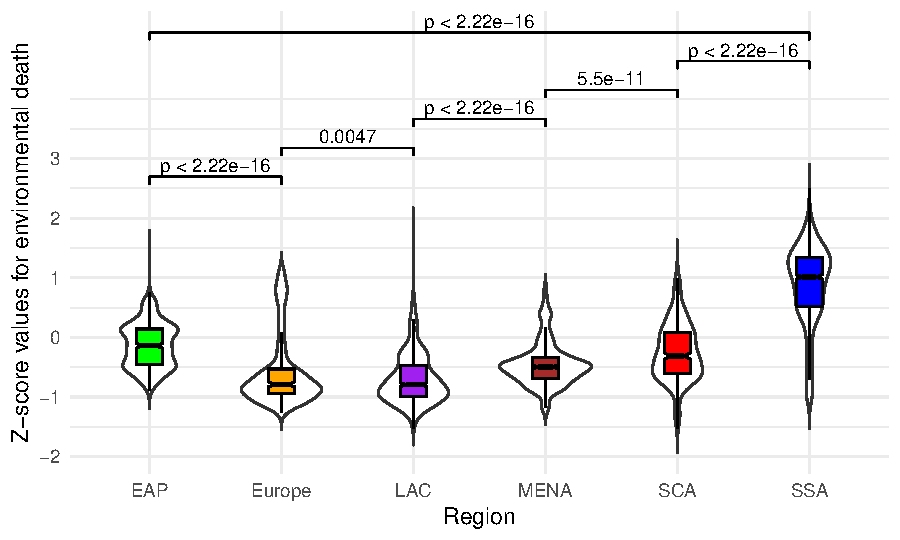
\includegraphics[width = 0.8\textwidth, height = 7cm]{Figures/Health_Outcome_Graph/Env_death_boxplt.pdf}
  %  \label{fig:Env mortality}
   % \caption*{\footnotesize{Note. Environmental mortality, as a dimension, comprises four mortality-based indicators: air pollution, unintentional poisoning, unclean water, and road traffic mortality. P-value derived from two-way paired t-test. All regions, except Europe and LAC, are significantly different. Author's computation, data from \textcite{unsdg_sustainable_2023, wdi_world_2023}}}
%\end{figure}




% Figure: Health System Capacity and Responsiveness
%Regardless of the intensity of health problems, health system capacity and responsiveness is essential to handle health problems when arise. Figure \ref{fig:Health syst Cap} shows all regions are statistically different in their level of health system capacity, even at p-value \textless{} 1\%.  Europe has the highest health capacity and responsiveness, with most of its countries clustering in the 75th quartile of its region. Both LAC and the MENA regions are also high in health capacity, with similar similar distribution shapes among their respective countries, clustering around the 75th percentile. While SCA and EAP regions also have somewhat similar, moderately better median values of health capacity, the distribution spreads out more among SCA countries than EAP. SSA has the poorest health system capacity and responsiveness among the regions \footnote{country level, refer to Appendix 8}.

%\begin{figure}[ht]
%\captionsetup{justification=justified,singlelinecheck=false}
%\caption{\textit{Health System Capacity and Responsiveness Dimension}}
 %   \centering 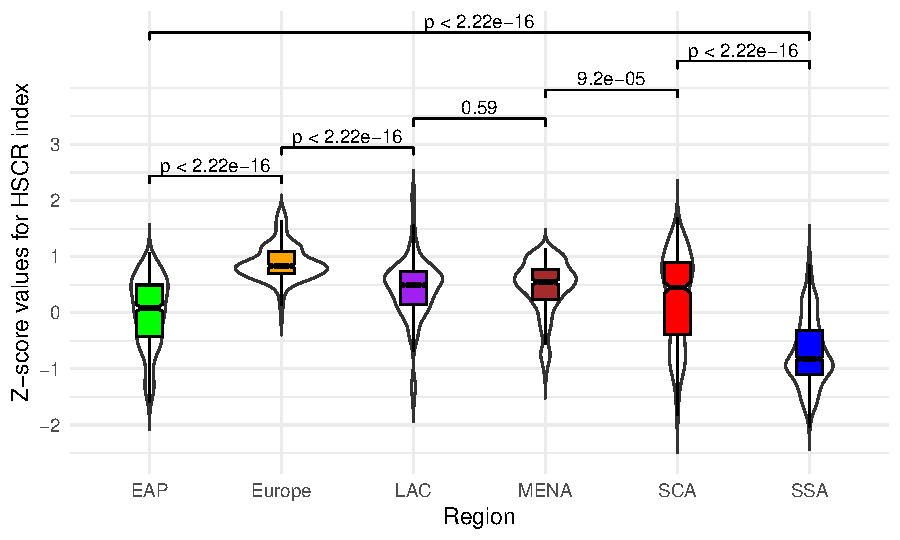
\includegraphics[width = 0.9\textwidth]{Figures/Health_Outcome_Graph/HSCR_Boxplt.pdf}
  %  \label{fig:Health syst Cap}
   % \caption{\footnotesize{Note. Health System Capacity and Responsiveness (HSCR) dimension is derived from six indicators: ODA devoted to health research and basic health activities, birth attended by skilled health personnel, population with access to measles second dose, health facility with essential medicine, health worker density, and family planning access rate. P-value derived from two-way paired t-test. All regions are significantly different at p-value \textless{} 1\%. Author's computation, data from \textcite{unsdg_sustainable_2023, wdi_world_2023}}}
%\end{figure}





%Figure: Health affordability and access
%As illustrated in Figure \ref{fig:CHS}, all regions exhibit a similar level of exposure, with varying levels of intensity distribution among their respective countries. However, the MENA region stands out with a higher incidence of CHS compared to others. CHS incidence is equally high in South and Central Asia (SCA), Europe, Latin America and the Caribbean (LAC), and East Asia and Pacific (EAP), each with a somewhat related nature of distribution among countries. Despite Sub-Saharan Africa (SSA) having the lowest incidence, with most of its countries clustering around the regional median, there are outliers, such as South Africa and Lesotho, with extreme values, ranking among the highest in the world.

%\begin{figure}[ht]    %\captionsetup{justification=justified,singlelinecheck=false}
 %   \caption{\textit{Affordability of Health Care Dimension}}
  %  \vspace{3pt}
   % \centering 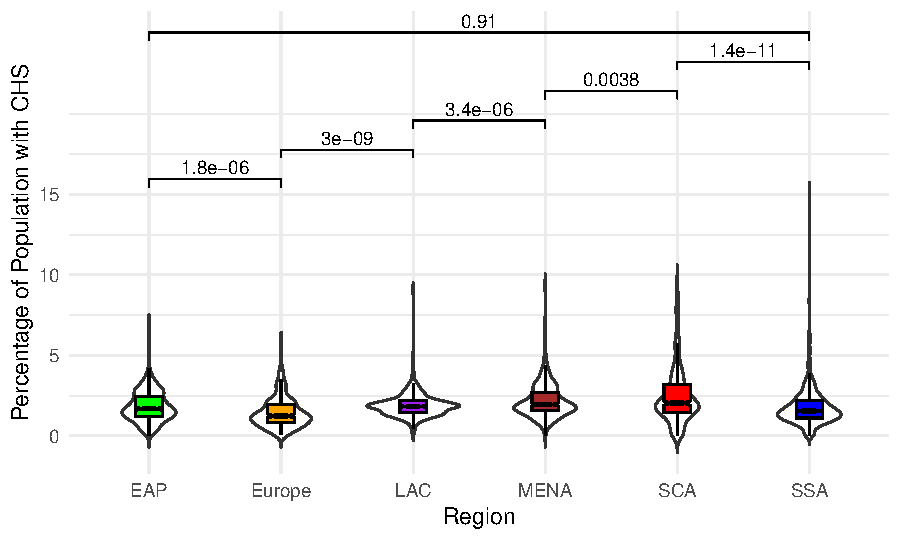
\includegraphics[width=0.8\textwidth, height=7cm]{Figures/Health_Outcome_Graph/CHS_boxplt.pdf}
    %\label{fig:CHS}
    %\caption*{\footnotesize{Note. This dimension is measured solely by the %proportion of the population with Catastrophic Health Spending (CHS) %\footnote{Scholars disagree on what amount of health expenditure %constitutes CHS. OOP \textgreater{} 25\% of household income is used in SDG 3 in line with \textcite{who_world_2010}. And it is adopted in this thesis}. All regions are significantly different at p-value \textless{} 1\%. Author's computation, data from \textcite{unsdg_sustainable_2023, wdi_world_2023}}}
%\end{figure}


Based on the preceding discussion, it is evident that regions exhibit significant differences across various health dimensions, reflecting diverse health situations. Consequently, relying solely on narrow health indicators to assess ODA effectiveness may lead to an underestimation of the intended impact. While the utilization of comprehensive health dimensions does not guarantee disparate results, it remains crucial for ensuring a valid and meaningful inter-region comparison


\subsection*{\quad 2.2.3 Does ODA Flow to Where it is most Needed?}
Previous studies, including \textcite{odokonyero_impact_2018, bavinger_relationship_2017, marty_taking_2017, temple_aid_2010}, have investigated the allocation patterns of foreign aid (ODA) in relation to health situations. In this thesis, a preliminary analysis deems it crucial to further explore the correlation between ODA allocation and various health dimensions. Figures \ref{fig:ODA against Hth dimension} and \ref{fig:Social Infrastructure scatterplt} in the appendix depict the relationship between the Log of ODA per GNI (ODA dependency) and social infrastructure ODA against different health dimensions. The objective is to discern whether countries facing the most significant health challenges receive higher foreign aid, particularly in the form of social infrastructure ODA. The two fitted lines, where the red line represents a linear regression fit and the black line signifies a nonlinear local projection fitted model in each scatterplot, provide insights into the direction and strength of the relationship. Notably, these plots are purely descriptive and are not intended to imply causality.

\begin{figure}[ht]
\captionsetup{justification=justified,singlelinecheck=false}
\caption{\textit{Relationship Between Total Net ODA and Health Dimensions}}
    \centering 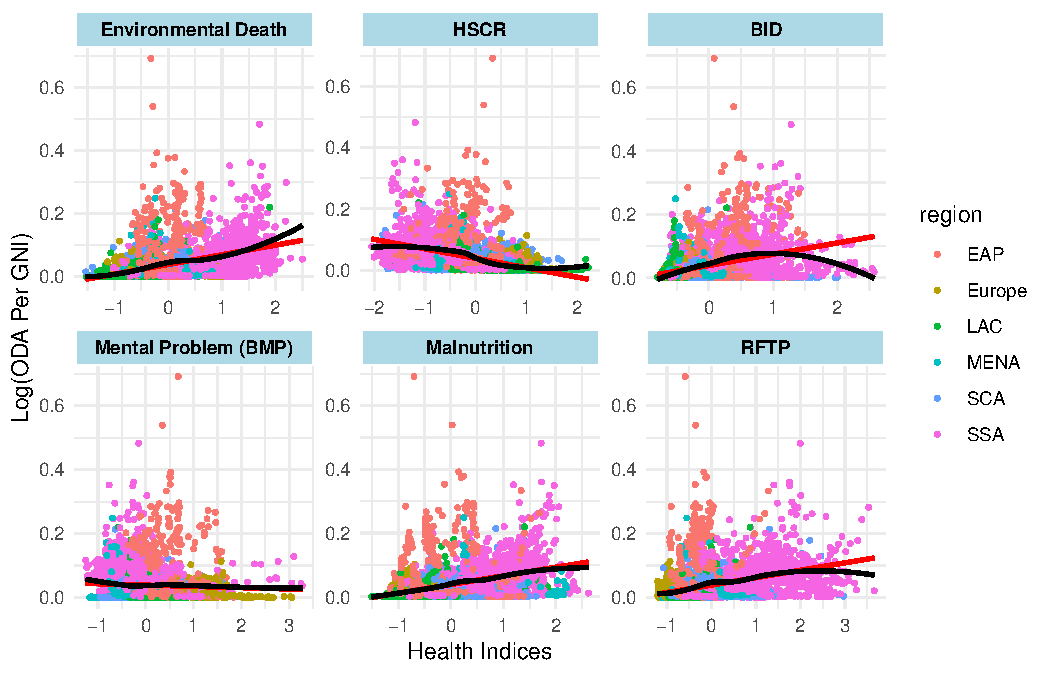
\includegraphics[width =  0.8\textwidth, height = 8cm]{Figures/ODA_against_Hth/ODA_Hth_plt.pdf}
    \label{fig:ODA against Hth dimension}
    \caption*{\footnotesize{Note: Author's computation, data from \textcite{unsdg_sustainable_2023, wdi_world_2023}}}
\end{figure}

From both Figure \ref{fig:ODA against Hth dimension} and Appendix Figure \ref{fig:Social Infrastructure scatterplt}, both total and social infrastructure exhibit a weak correlation and slightly different pattern of relationship across the six health dimensions. Against the position of \textcite{temple_aid_2010}, the finding is supported by a range of others, including \textcite{odokonyero_impact_2018, bavinger_relationship_2017, marty_taking_2017}, who have all argued that ODA flows to where it is less needed. Furthermore, the divergence between the two fitted lines indicates that the relationship between ODA and health problems is not linear. In other words, the flow of ODA does not consistently depend on the burden of health problems. While this suggests a weak statistical association, it does not imply causation.  


%The results revealed a weak negative correlation between ODA across all health dimensions, with correlation coefficients from -0.6 on mental health to 0.30 on under-nutrition (p \textless{} 0.05). 




\subsection*{2.3 Social protection} 
\addcontentsline{toc}{subsection}{2.3 Social protection}
\subsubsection*{\quad 2.3.1 Conceptualizing Social protection}
\addcontentsline{toc}{subsubsection}{2.3.1 Conceptualizing Social protection}
Social protection is a multifaceted concept, shaped by diverse socio-cultural contexts and evolving social risks \parencite{yokobori_roles_2023}. Hence, there is no universally accepted definition and measurement of social protection. The International Labour Organization (ILO), for instance, define social protection as a combination of policies and programs aimed at reducing and preventing poverty and vulnerability throughout the life cycle \parencite[see][]{yokobori_roles_2023, ilo_social_2012}. The ILO Social Protection Floor (SPF), in particular, characterizes social protection as set of minimum social security guarantees, nationally defined to forestall or alleviate poverty, vulnerability, and social exclusion \parencite{ilo_social_2012}. The World Bank, adopting an empowerment approach, defines social protection as a system to help vulnerable individuals cope with life's shocks  and capacity to protect themselves against such shocks \parencite[Discussion in][]{yokobori_roles_2023}. This definition is deeply rooted in Social Risk Management (SRM), viewing social protection as a tool for risk prevention, management, and coping \parencite[]{holzmann_social_2001}.

More succinctly, \textcite{midgley_advanced_2022} defines social protection as resource transfers to individuals or households, ensuring current or future income security. Social protection employs various means, broadly categorized into social assistance, social insurance, and labor market programs, implemented through national policies, international organizations, NGOs, and other authorized state and non-state institutions \parencite{holzmann_social_2001, midgley_advanced_2022, yokobori_roles_2023}. Despite the diverse definitions and functions of social protection, the availability of suitable social protection data for panel analysis poses a challenge \parencite{nino-zarazua_aids_2023}. Given the lack of sufficient panel data for social protection, this thesis utilizes the World Bank ASPIRE data on the total social protection coverage as percentage of population \parencite{wdi_world_2023}, for further analysis.


%social protection development is proxy by the social protection floor, an initiative of the ILO known as Recommendation 202. This framework defines the social protection floor as a set of basic social security guarantees, nationally defined to prevent or alleviate poverty, vulnerability, and social exclusion \parencite{ilo_social_2012}. The framework recommends four minimum levels of social security within national capacities, spanning the lifecycle: access to healthcare, including maternity care; basic child income security; basic active age income security; and basic income security for the older population \parencite{ilo_social_2012}. This framework has been integrated into global development commitments, notably SDG 1.3, leading to the establishment of eight indicators measuring different dimensions of the social protection floor, including the coverage of respective programs outlined in Recommendation 202. The subsequent section provides a descriptive explanation of the distribution of social protection floor indicators.

\subsubsection*{\quad 2.3.2  Social Protection}
\addcontentsline{toc}{subsubsection}{2.3.2 Evolution of Social Protection Development}
\begin{figure}[ht]
\caption{\textit{Relationship Between Social Protection Coverage and Health Dimensions}}
    \centering 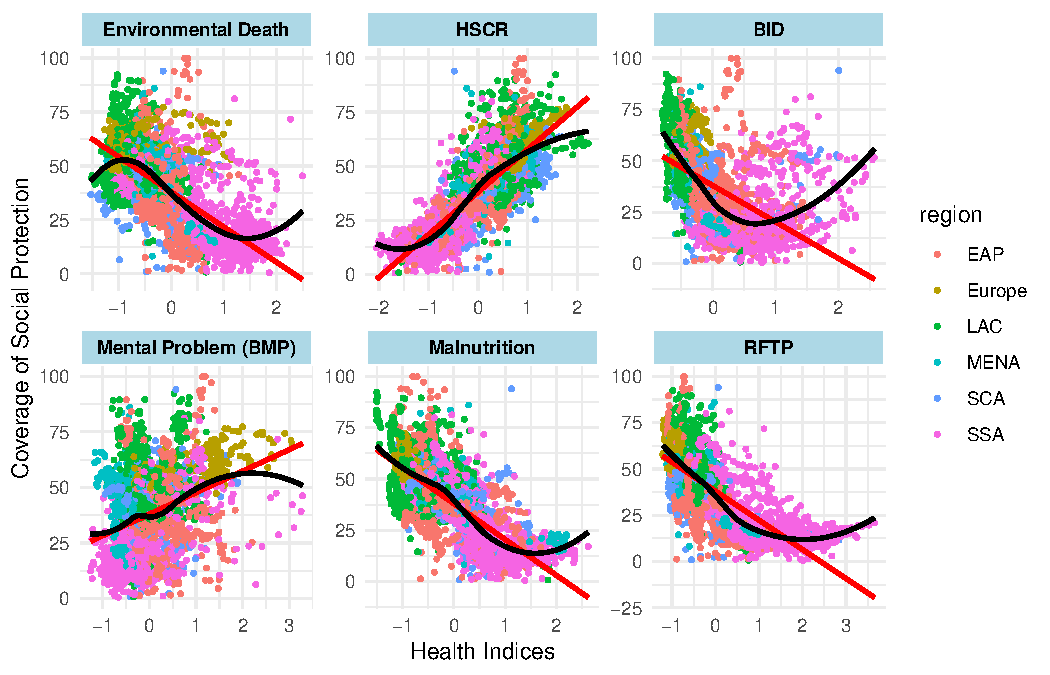
\includegraphics[width = 0.8\textwidth]{Figures/ODA_against_Hth/SocProct_Hlth_plt.pdf}
    \caption*{\footnotesize Note: Social protection coverage is in \% of the total population. Red and black fitted lines are linear and non-linear respectively. Author's computation, data from \textcite{unsdg_sustainable_2023, wdi_world_2023}}
    \label{Fig::SocailProtection and Health}
\end{figure}

The section explains the dynamics of relationship between social protection, health dimensions, and ODA, as shown in Figure \ref{Fig::SocailProtection and Health}, and Appendix Figure \ref{Fig::Social_Prot_Total_ODA} and \ref{Fig::Social_Prot_Social_InfrastructureODA}. Figure \ref{Fig::SocailProtection and Health} shows clear relationship between social protection and various health dimensions. The observed relationship tends to exhibit a non-linear trend, as evidenced by the fitted black lines in Figure \ref{Fig::SocailProtection and Health}. Conversely, in the Appendix Figure \ref{Fig::Social_Prot_Total_ODA} and \ref{Fig::Social_Prot_Social_InfrastructureODA}, neither total net ODA nor social infrastructure ODA  manifests a clear relationship with social protection coverage. It is important to note that this preliminary analysis suggests a potential influence of social protection on health dimensions, with weak evidence on the relationship ODA and social protection. While these graphs are mere descriptive, it does not imply causality. This hypothesis will be further examined and tested  in the subsequent chapters of the thesis.



\subsubsection*{2.4  Conclusion and Summary from Preliminary Analysis}
In essence, the preliminary analysis chapter delves into the complex interplay between the allocation patterns of Official Development Assistance (ODA), health dimensions, and social protection.

\begin{itemize}
    \item The chapter reveal ODA allocation varies with time and reflects global situations. Moreover, Africa and Asia have been the highest recipient of ODA with the United States (US) and Germany being the highest and most predictable donors. Additionally, countries in East Asia and the Pacific (EAP) and Sub-Saharan Africa tend to be more aid-dependent than others. 
    \item By leveraging comprehensive health dimensions, the chapter unveils substantial variations in health situations across regions. Specifically, while reproductive fatality, infection and diseases as well as environmental death are prevalent in SSA, SCA and EAP, mental problem is the major problem in Europe. Moreover, Europe has the best health system capacity, with SSA region being the poorest in this respect. 
    \item The analysis reveals that ODA allocation does not necessarily align with the health needs of recipient countries. 
    \item Finally, While social protection tend to have clear and discernible relationship with all health dimensions, ODA as weak relationship with social protection. While the preliminary offers hint on the pattern of relationship, it does not imply causality. All hypotheses are further tested in the main analysis in Chapter Five. 
\end{itemize}
    
%   The examination of ODA recipients highlights the consistent prominence of Africa, followed closely by Asia, while also emphasizing that the distribution of aid doesn't always align precisely with the regions facing the most pressing health needs.

%Crucially, these findings prompt a reflection on the alignment of international aid with the identified health needs. Our preliminary analysis, as depicted in Figure \ref{fig:ODA against Hth dimension}, \ref{fig:Social Infrastructure scatterplt} and \ref{fig:preliminary stat pair panels}, explores the relationship between ODA allocation and health outcomes. While certain dimensions exhibit a discernible association with ODA, the complex interplay suggests that foreign aid distribution is not solely determined by the magnitude of health challenges in a given region. 

%This insight contributes to the broader investigation into whether foreign aid effectively targets regions with the greatest health needs, as posed in the central research question of the thesis. The nuanced nature of the relationships underscores the multifaceted considerations involved in international aid allocation and sets the stage for a more in-depth exploration in subsequent sections.
